%%%%%%%%%%%%  Generated using docx2latex.pythonanywhere.com  %%%%%%%%%%%%%%


\documentclass[a4paper,12pt]{report}

% Other options in place of 'report' are 1)article 2)book 3)letter
% Other options in place of 'a4paper' are 1)a5paper 2)b5paper 3)letterpaper 4)legalpaper 5)executivepaper


 %%%%%%%%%%%%  Include Packages  %%%%%%%%%%%%%%


\usepackage{amsmath}
\usepackage{latexsym}
\usepackage{amsfonts}
\usepackage{amssymb}
\usepackage{graphicx}
\usepackage{txfonts}
\usepackage{wasysym}
\usepackage{enumitem}
\usepackage{adjustbox}
\usepackage{ragged2e}
\usepackage{tabularx}
\usepackage{changepage}
\usepackage{setspace}
\usepackage{hhline}
\usepackage{multicol}
\usepackage{float}
\usepackage{multirow}
\usepackage{makecell}
\usepackage{fancyhdr}
\usepackage[toc,page]{appendix}
\usepackage[utf8]{inputenc}
\usepackage[T1]{fontenc}
\usepackage{hyperref}


 %%%%%%%%%%%%  Define Colors For Hyperlinks  %%%%%%%%%%%%%%


\hypersetup{
colorlinks=true,
linkcolor=blue,
filecolor=magenta,
urlcolor=cyan,
}
\urlstyle{same}


 %%%%%%%%%%%%  Set Depths for Sections  %%%%%%%%%%%%%%

% 1) Section
% 1.1) SubSection
% 1.1.1) SubSubSection
% 1.1.1.1) Paragraph
% 1.1.1.1.1) Subparagraph


\setcounter{tocdepth}{5}
\setcounter{secnumdepth}{5}


 %%%%%%%%%%%%  Set Page Margins  %%%%%%%%%%%%%%


\usepackage[a4paper,bindingoffset=0.2in,headsep=0.5cm,left=1.0in,right=1.0in,bottom=2cm,top=2cm,headheight=2cm]{geometry}
\everymath{\displaystyle}


 %%%%%%%%%%%%  Set Depths for Nested Lists created by \begin{enumerate}  %%%%%%%%%%%%%%


\setlistdepth{9}
\newlist{myEnumerate}{enumerate}{9}
	\setlist[myEnumerate,1]{label=\arabic*)}
	\setlist[myEnumerate,2]{label=\alph*)}
	\setlist[myEnumerate,3]{label=(\roman*)}
	\setlist[myEnumerate,4]{label=(\arabic*)}
	\setlist[myEnumerate,5]{label=(\Alph*)}
	\setlist[myEnumerate,6]{label=(\Roman*)}
	\setlist[myEnumerate,7]{label=\arabic*}
	\setlist[myEnumerate,8]{label=\alph*}
	\setlist[myEnumerate,9]{label=\roman*}

\renewlist{itemize}{itemize}{9}
	\setlist[itemize]{label=$\cdot$}
	\setlist[itemize,1]{label=\textbullet}
	\setlist[itemize,2]{label=$\circ$}
	\setlist[itemize,3]{label=$\ast$}
	\setlist[itemize,4]{label=$\dagger$}
	\setlist[itemize,5]{label=$\triangleright$}
	\setlist[itemize,6]{label=$\bigstar$}
	\setlist[itemize,7]{label=$\blacklozenge$}
	\setlist[itemize,8]{label=$\prime$}



 %%%%%%%%%%%%  Header here  %%%%%%%%%%%%%%


\pagestyle{fancy}
\fancyhf{}


 %%%%%%%%%%%%  Footer here  %%%%%%%%%%%%%%




 %%%%%%%%%%%%  Print Page Numbers  %%%%%%%%%%%%%%


\rfoot{\thepage}


 %%%%%%%%%%%%  This sets linespacing (verticle gap between Lines) Default=1 %%%%%%%%%%%%%%


\setstretch{1.08}


 %%%%%%%%%%%%  Document Code starts here %%%%%%%%%%%%%%


\begin{document}
\sloppy
\begin{center}{\fontsize{14pt}{14pt}\selectfont \textbf{DATABASE ACCESS} \\}\end{center} \par
\noindent 
\textbf{Pengertian Database} \par
Basis data adalah sekumpulan dari data yang telah disusun sesuai dengan aturan tertentu yang saling berhubungan sehingga memudahkan pengguna dalam mengelolanya juga memudahkan pengguna untuk memperoleh informasi. Selain itu ada juga yang menyebutkan bahwa database sebagai kumpulan file, tabel, atau arsip yang saling terhubung yang disimpan dalam media elektronik.  \par
\vspace{12pt}
\noindent 
\textbf{Manfaat Penggunaan Database} \par
\noindent 
\begin{myEnumerate}
\item Kecepatan dan Kemudahan \par
Database memiliki kemampuan dalam menyeleksi data sehingga menjadi suatu kelompok yang tersusun dengan cepat. Hal inilah yang ahirnya dapat menghasilkan informasi yang dibutuhkan secara cepat pula. Seberapa cepat pemrosesan data oleh database tergantung pada perancangan databasenya. \par
\vspace{12pt}
\noindent 
\item Pemakaian Bersama-sama \par
Suatu database bisa digunakan oleh siapa saja dalam suatu perusahaan. Sebagai contoh database mahasiswa dalam suatu perguruan tinggi dibutuhkan oleh beberapa bagian, seperti bagian admin, bagian keuangan, bagian akademik. Kesemua bidang tersebut membutuhkan database mahasiswa namun tidak perlu masing-masing bagian membuat databasenya sendiri, cukup database mahasiswa satu saja yang disimpan di server pusat. Nanti aplikasi dari masing-masing bagian bisa terhubung ke database mahasiswa tersebut. \par
\vspace{12pt}
\noindent 
\item Kontrol data terpusat \par
Masih berkaitan dengan point ke dua, meskipun pada suatu perusahaan memiliki banyak bagian atau divisi tapi database yang diperlukan tetap satu saja. Hal ini mempermudah pengontrolan data seperti ketika ingin mengupdate data mahasiswa, maka kita perlu mengupdate semua data di masing-masing bagian atau divisi, tetapi cukup di satu database saja yang ada di server pusat. \par
\vspace{12pt}
\vspace{12pt}
\noindent 
\item Menghemat biaya perangkat \par
Dengan memiliki database secara terpusat maka di masing-masing divisi tidak memerlukan perangkat untuk menyimpan database berhubung database yang dibutuhkan hanya satu yaitu yang disimpan di server pusat, ini tentunya memangkas biaya pembelian perangkat. \par
\vspace{12pt}
\noindent 
\item Keamanan Data \par
Hampir semua Aplikasi manajemen database sekarang memiliki fasilitas manajemen pengguna. Manajemen pengguna ini mampu membuat hak akses yang berbeda-beda disesuaikan dengan kepentingan maupun posisi pengguna. Selain itu data yang tersimpan di database diperlukan password untuk mengaksesnya. \par
\vspace{12pt}
\noindent 
\item Memudahkan dalam pembuatan Aplikasi baru\end{myEnumerate}
 \par
Dalam poin ini database yang dirancang dengan sangat baik, sehingga si perusahaan memerlukan aplikasi baru tidak perlu membuat database yang baru juga, atau tidak perlu mengubah kembali struktur database yang sudah ada. Sehingga Si pembuat aplikasi atau programmer hanya cukup membuat atau pengatur antarmuka aplikasinya saja. \par
\vspace{12pt}
Dengan segudang manfaat dan kegunaan yang dimiliki oleh database maka sudah seharusnya semua perusahaan baik itu perusahaan skala kecil apalagi perusahaan besar memilki database yang dibangun dengan rancangan yang baik. Ditambah dengan pemanfaatan teknologi jaringan komputer maka manfaat database ini akan semakin besar. Penggunaan database sekaligus teknologi jaringan komputer telah banyak digunakan oleh berbagai macam perusahaan, contohnya saja perbankan yang memiliki cabang di setiap kotanya. Perusahaan Bank tersebut hanya memiliki satu database yang disimpan di server pusat, sedangkan cabang-cabangnya terhubung melalui jaringan komputer untuk mengakses database yang terletak di sever pusat tersebut. \par
\vspace{12pt}
\vspace{12pt}
\vspace{12pt}
\noindent 
\textbf{Apa yang dimaksud dengan}\textbf{ field, record, }\textbf{table, file, data  $  \&  $ basis data?} \par
Field merupakan kumpulan dari karakter yang membentuk satu arti, maka jika terdapat field misalnya seperti KeteranganBarang atau JumlahBarang, maka yang dimunculkan dalam field tersebut harus yang berkaitan dengan keterangan barang dan jumlah barang. Atau field juga bisa disebut sebagai tempat atau kolom yang terdapat dalam suatu tabel untuk mengisikan nama-nama (data) field yang akan di isikan. \par
\vspace{12pt}
Record merupakan kumpulan field yang sangat lengkap, dan biasanya dihitung dalam satuan baris. Tabel merupakan kumpulan dari beberapa record dan juga field. File terdiri dari kumpulan field yang menunjukan dari satu kesatuan data yang sejenis. Misalnya seperti file nama siswa berisikan data tentang semua nama siswa yang ada. Data adalah kumpulan fakta atau kejadian yang digunakan sebagai penyelesaian masalah dalam bentuk informasi. Basis data (database) terdiri dari dua kata, yaitu kata basis dan data. Basis merupakan tempat ataupun gudang, maupun wadah. \par
\vspace{12pt}
\noindent 
\begin{center}

 %%%%%%%%%%%%  Figure/Image No:1 here %%%%%%%%%%%%%%


\begin{figure}[H]
\begin{center}
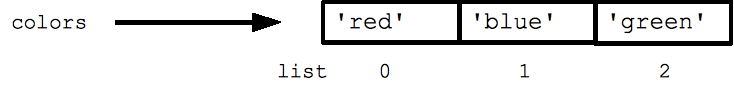
\includegraphics[width=4.63in,height=2.0in]{./uploads_new/DATABASE_ACCESS.docx_DIR/media/image1.png}
\end{center}
\end{figure}


 %%%%%%%%%%%%  Figure/Image No:1 Ends Here %%%%%%%%%%%%%%


\end{center}\vspace{12pt}
\vspace{12pt}
Data dapat disebut sebagai kumpulan dari fakta yang mewakili objek, misalnya seperti benda, manusia,barang dan sebagainya yang ditulis ke dalam bentuk angka, huruf, simbol, bunyi, teks, gambar ataupun gabungannya. Jadi dapat disimpulkan bahwa basis data merupakan kumpulan dari data-datayang terorganisasi yang saling berhubungan sedemikian rupa sehingga dapat dengan mudah disimpan, dimanipulasi, dan dipanggil oleh pemakainya. Karakter atau character yang ada didalam database merupakan bagian data yang terkecil, karakter tersebutdapat berupa karakter numerik, huruf ataupun karakter khusus (special characters) yang membentuk suatu item data atau field. \par
\vspace{12pt}
\noindent 
\textbf{Sifat-sifat database / basis data} \par
\noindent 
\begin{itemize}
\item Internal~~~~~~~~:  kesatuan (integritas) dari file-file yang terlibat \par
\noindent 
\item Terbagi/share : elemen-elemen database dapat dibagikan pada para user baik secara sendiri-sendiri maupun secara serentak dan pada waktu yang sama (concurrent sharing).\end{itemize}
 \par
\vspace{12pt}
\noindent 
\textbf{Tipe Database / basis data} \par
\noindent 
Tipe Database Terdapat 12 tipe database, antara lain: \par
\noindent 
\begin{myEnumerate}
\item Operational database: Database ini menyimpan data rinci yang diperlukan untuk mendukung operasi dari seluruh organisasi. Mereka juga disebut subject-area databases (SADB), transaksi database, dan produksi database. Contoh: database pelanggan, database pribadi, database inventaris, akuntansi database. \par
\noindent 
\item Analytical database: Database ini menyimpan data dan informasi yang diambil dari operasional yang dipilih dan eksternal database. Mereka terdiri dari data dan informasi yang dirangkum paling dibutuhkan oleh sebuah organisasi manajemen dan End-user lainnya. Beberapa orang menyebut analitis multidimensi database sebagai database, manajemen database, atau informasi database. \par
\noindent 
\item Data warehouse: Sebuah data warehouse menyimpan data dari saat ini dan tahun- tahun sebelumnya - data yang diambil dari berbagai database operasional dari sebuah organisasi. \par
\noindent 
\item Distributed database: Ini adalah database-kelompok kerja lokal dan departemen di kantor regional, kantor cabang, pabrik-pabrik dan lokasi kerja lainnya. Database ini dapat mencakup kedua segmen yaitu operasional dan user database, serta data yang dihasilkan dan digunakan hanya pada pengguna situs sendiri. \par
\noindent 
\item End-user database: Database ini terdiri dari berbagai file data yang dikembangkan oleh end-user di workstation mereka. Contoh dari ini adalah koleksi dokumen dalam spreadsheet, word processing dan bahkan download file. \par
\noindent 
\item External database: Database ini menyediakan akses ke eksternal, data milik pribadi online - tersedia untuk biaya kepada pengguna akhir dan organisasi dari layanan komersial. Akses ke kekayaan informasi dari database eksternal yang tersedia untuk biaya dari layanan online komersial dan dengan atau tanpa biaya dari banyak sumber di Internet. \par
\noindent 
\item Hypermedia databases on the web: Ini adalah kumpulan dari halaman-halaman multimedia yang saling berhubungan di sebuah situs web. Mereka terdiri dari home page dan halaman hyperlink lain dari multimedia atau campuran media seperti teks, grafik, gambar foto, klip video, audio dll. \par
\noindent 
\item Navigational database: Dalam navigasi database, queries menemukan benda terutama dengan mengikuti referensi dari objek lain. \par
\noindent 
\item In-memory databases: Database di memori terutama bergantung pada memori utama untuk penyimpanan data komputer. Ini berbeda dengan sistem manajemen database yang menggunakan disk berbasis mekanisme penyimpanan. Database memori utama lebih cepat daripada dioptimalkan disk database sejak Optimasi algoritma internal menjadi lebih sederhana dan lebih sedikit CPU mengeksekusi instruksi. \par
\noindent 
\item Document-oriented databases: Merupakan program komputer yang dirancang untuk aplikasi berorientasi dokumen. Sistem ini bisa diimplementasikan sebagai lapisan di atas sebuah database relasional atau objek database. Sebagai lawan dari database relasional, dokumen berbasis database tidak menyimpan data dalam tabel dengan ukuran seragam kolom untuk setiap record. Sebaliknya, mereka menyimpan setiap catatan sebagai dokumen yang memiliki karakteristik tertentu. Sejumlah bidang panjang apapun dapat ditambahkan ke dokumen. Bidang yang dapat juga berisi beberapa bagian data. \par
\noindent 
\item Real-time databases Real-time: Database adalah sistem pengolahan dirancang untuk menangani beban kerja negara yang dapat berubah terus- menerus. Ini berbeda dari database tradisional yang mengandung data yang terus- menerus, sebagian besar tidak terpengaruh oleh waktu. \par
\noindent 
\item Relational Database: Database yang paling umum digunakan saat ini. Menggunakan meja untuk informasi struktur sehingga mudah untuk mencari.\end{myEnumerate}
 \par
\vspace{12pt}
\noindent 
\textbf{Modul python}\textbf{ untuk mengakses database MySQL} \par
Untuk mengakses database MySQL dari Python, berikut adalah beberapa langkah sederhana. Yang pertama, server database MySQL harus siap dulu. Karenanya lakukan tahapan berikut ini. \par
\noindent 
\begin{myEnumerate}
\item Instal server mysql dengan menjalankan perintah sudo apt-get install mysql-server. Jangan lupa memasukkan password akun root untuk server MySQL. \par
\noindent 
\item Siapkan database dan tabel. Jalankan perintah mysql -u root -p dari terminal. Selanjutnya, kita akan masuk ke shell MySQL. Selanjutnya kita akan buat tabel yang skemanya seperti berikut ini (hanya ilustrasi saja). \par
mysql> create database teman; \par
mysql> use teman; \hspace*{1.69in}  \par
mysql> create table alamat(id int not null auto $  \_  $increment primary key, nama varchar(35), alamat text, telepon varchar(15), surat text); \par
\vspace{12pt}
\noindent 
\item  ingin membuat user baru yang punya akses penuh ke database yang baru saja dibuat, lakukan tahapan berikut ini. \par
mysql> create user 'andri'@'localhost' identified by '123456'; \par
mysql> grant all on teman.* to 'andri'@'localhost' with grant option; \par
\noindent 
\item Langkah selanjutnya adalah membuat modul python untuk mengakses database tersebut. Untuk kasus ini, modul hanya diberi kemampuan untuk melihat seluruh isi tabel, sehingga tabel sebaiknya diisi dulu. Sedangkan kemampuan untuk melakukan operasi update dan delete dapat dibangun menggunakan pola yang sama. Modul tersebut seperti code berikut.\end{myEnumerate}
 \par
\vspace{12pt}
Modul terdiri dari dua fungsi, masing-masing sambung dan selectall. Fungsi pertama membutuhkan parameter terkait nama server, dan akun user serta mengembalikan variabel koneksi. Sedangkan fungsi selectall membutuhkan parameter koneksi yang diperoleh dari fungsi sambung, serta nama database dan nama tabel. Fungsi ini mengembalikan list yang berisi setiap row dalam tabel untuk kebutuhan lain yang belum terdefinisi dalam modul ini. \par
\vspace{12pt}
\noindent 
import MySQLdb \par
\noindent 
def sambung (host,user,passwd): \par
\noindent 
~ mycon=MySQLdb.connect(host,user,passwd) \par
\noindent 
~ return mycon \par
\vspace{12pt}
\noindent 
def selectall(mycon, dbname, table): \par
\noindent 
~ mycur=mycon.cursor() \par
\noindent 
~ mycur.execute('use ' + dbname) \par
\noindent 
~ mycur.execute('select * from ' + table) \par
\noindent 
~ rows=mycur.fetchall() \par
\noindent 
~ a=[] \par
\noindent 
~ for i in rows: \par
\noindent 
~~~ nama=i[1] \par
\noindent 
~~~ alamat=i[2] \par
\noindent 
~~~ telepon=i[3] \par
\noindent 
~~~ surat=i[4] \par
\noindent 
~~~ print(nama + ' ' + alamat + ' ' + telepon + ' ' + surat) \par
\noindent 
~~~ a.append(i) \par
\noindent 
~ return a \par
Lalu, bagaimana menggunakannya? Untuk sementara, modul python ini hanya dapat diakses melalui shell python karena belum ada fungsi main yang terdefinsi. Hal ini disebabkan karena rancangan input/ouput masih seadanya. Karenanya, mari masuk ke shell python dengan menjalankan perintah python di terminal. Yang perlu diperhatikan, penggunaan shell python harus dilakukan dari directory di mana modul ini disimpan. Berikut adalah gambaran ketika berada dalam shell python dan menggunakan modul ini. \par
\noindent 
>>> from mymodul import * \par
\noindent 
>>> mycon=sambung("localhost","andri","123456") \par
\noindent 
>>> a=selectall(mycon,"teman","alamat") \par
\noindent 
Andri Jl. Sariasih, Sarijadi, Bandung 12450 08123456789 andri@poltekpos.ac.id \par
\noindent 
>>> \par
Di baris pertama, kita meng-import modul dari nama file, untuk selanjutnya meng-import semua fungsi yang ada di dalamnya. Selanjutnya, kita membuat variabel bernama mycon bertipe koneksi ke MySQL (dapat dilihat dengan cara menjalankan perintah type(mycon) dari shell python) dan meng-assigned nilainya dari memanggil fungsi sambung. Selanjutnya, variabel a di-assinged nilainya dari memanggil fungsi selectall. Terlihat bahwa fungsi selectall mencetak nilai yang diperoleh dari operasi select tabel. \par
\vspace{12pt}
Dengan ilustrasi ini, diharapkan dapat memberi inspirasi membuat modul python yang digunakan untuk sebuah aplikasi, misalnya dengan menjadikannya sebagai bagian dari hubungan SIGNAL-SLOT pada QT4. Semoga bermanfaat. \par
\vspace{12pt}
Dalam era informasi dimana kita hidup sekarang, kita dapat melihat seberapa banyak data dunia berubah. Kita pada dasarnya membuat, menyimpan, dan menarik data, secara ekstensif! Harusnya ada sebuah cara untuk menangani semua itu—itu tidak dapat disebarkan kemana-mana tanpa adanya manajemen bukan? Di sini hadir Database Management System (DBMS). DBMS adalah sebuah sistem software yang memungkinkanmu untuk membuat, menyimpan, memodifikasi, menarik, dan penanganan lainnya terhadap sebuah data dari database. Sistem ini juga bervariasi dalam ukuran, mulai dari sistem kecil yang cukup berjalan pada komputer personal hingga yang lebih besar yang berjalan dalam mainframe. \par
\vspace{12pt}
\noindent 
\textbf{Python Database API} \par
Python dapat berinteraksi dengan database. Namun, bagaimana itu dapat melakukannya? Python menggunakan apa yang disebut Python Database API dengan tujuan untuk menjadi antarmuka dengan database. API ini mengijinkan kita untuk memprogram database management system (DBMS) yang berbeda. Untuk DBMS yang berbeda itu, bagaimana pun juga, proses yang diikuti pada tingkatan code tetap sama, yaitu sebagai berikut: \par
\vspace{12pt}
\noindent 
\begin{itemize}
\item Membangun sebuah koneksi ke database pilihanmu. \par
\noindent 
\item Membuat sebuah kursor untuk berkomunikasi dengan data. \par
\noindent 
\item Memanipulasi data menggunakan SQL (berinteraksi). \par
\noindent 
\item Memberitahu koneksi untuk entah menerapkan manipulasi SQL ke data dan membuatnya permanen (commit), atau memberitahunya untuk meninggalkan manipulasi itu (rollback), sehingga mengembalikan data ke keadaan sebelum interaksi terjadi. \par
\noindent 
\item Menutup koneksi ke database.\end{itemize}
 \par
Bagaimana caranya menampilkan data dari mysql menggunakan python. Saya asumsikan teman-teman sudah menginstall web server (XAMPP/yang lainnya) dan python di komputer masing-masing. Setelah itu semua siap sekarang silahkan download mysql connector untuk python disini (Sesuaikan dengan versi python yang kalian punya). Setelah itu tinggal install. \par
Setelah selesai installasi, buka phpmyadmin dan buat database dengan nama terserah. Contohnya yaitu  $ " $trial $ " $ Lalu import sql berikut \par
\noindent 
trial.sql \par
\noindent 
Setelah di impor, lalu buka teks editor dan copas-kan code berikut \par
\noindent 
show-data.py \par
\noindent 
lalu simpan dengan nama terserah kalian (punya saya show-data.py) dan tinggal kalian run dari command prompt. \par
\vspace{12pt}
\noindent 
\textbf{Koneksi Database MySQL dengan Python} \par
\noindent 
\begin{myEnumerate}
\item Pastikan sudah mengintal package libmysqlclient-dev dengan: \par
apt-get install libmysqlclient-dev \par
\noindent 
\item Download modul MySQLdb. \par
\noindent 
\item Instal modul tersebut dengan cara (Pastikan login sebagai root ya): \par
 $  \$  $ gunzip MySQL-python-1.2.2.tar.gz \par
 $  \$  $ tar -xvf MySQL-python-1.2.2.tar \par
 $  \$  $ cd MySQL-python-1.2.2 \par
 $  \$  $ python setup.py build \par
 $  \$  $ python setup.py install \par
\noindent 
\item Buat satu script seperti berikut (contoh: test.py): \par
import MySQLdb \par
 $  \#  $ Open database connection \par
db = MySQLdb.connect("localhost","root","password","nama $  \_  $database" ) \par
 $  \#  $ prepare a cursor object using cursor() method \par
cursor = db.cursor() \par
 $  \#  $ execute SQL query using execute() method. \par
cursor.execute("SELECT VERSION()") \par
 $  \#  $ Fetch a single row using fetchone() method. \par
data = cursor.fetchone() \par
print "Database version :  $  \%  $s "  $  \%  $ data \par
 $  \#  $ disconnect from server \par
db.close() \par
\noindent 
\item Test dengan code berikut:\end{myEnumerate}
 \par
python test.py \par
\vspace{12pt}
\end{document}
